\begin{figure}[H]
    \begin{subfigure}[t]{.45\textwidth}
        \caption{}
        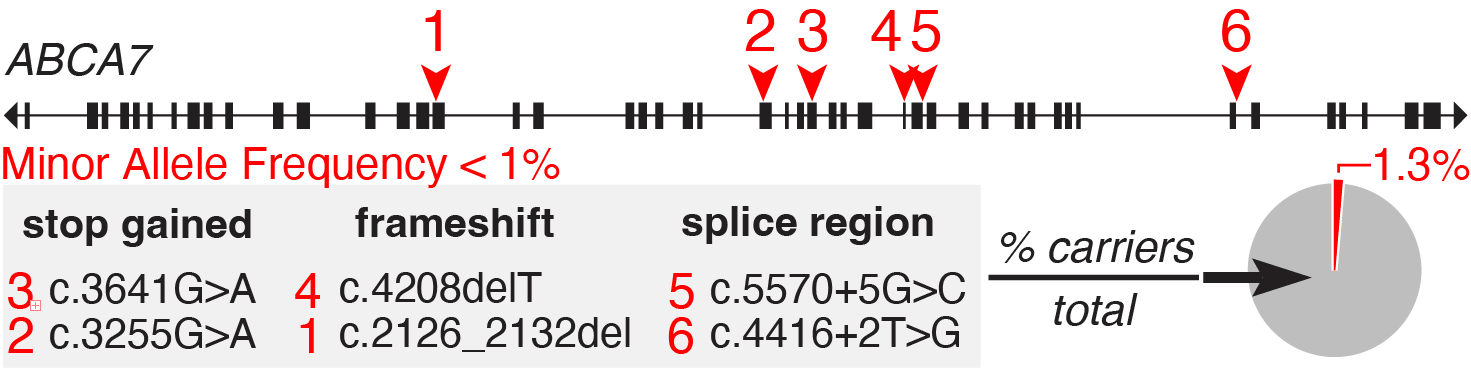
\includegraphics[width=\textwidth]{./main_plots/abca7_variants_cartoon.png}        
    \end{subfigure}
    \begin{subfigure}[t]{.55\textwidth}
        \caption{}
        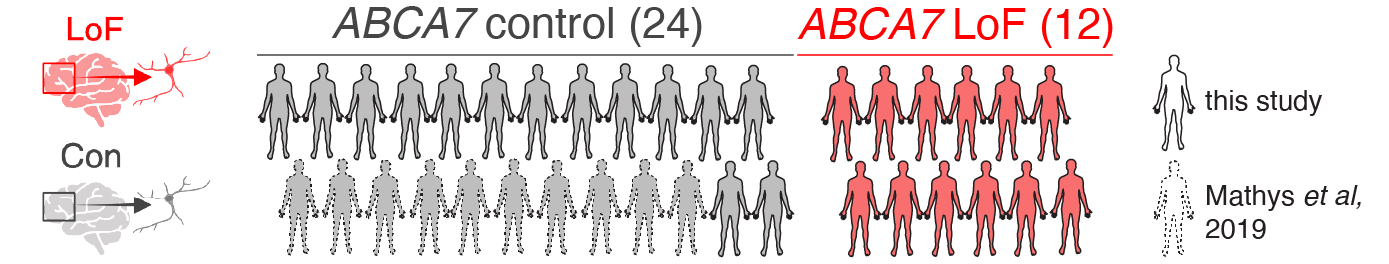
\includegraphics[width=\textwidth]{./main_plots/cohort_cartoon.png}        
    \end{subfigure}
    \\[-1ex] 
    \begin{subfigure}[t]{.5\textwidth}
        \begin{subfigure}[t]{\textwidth}
            \caption{}
            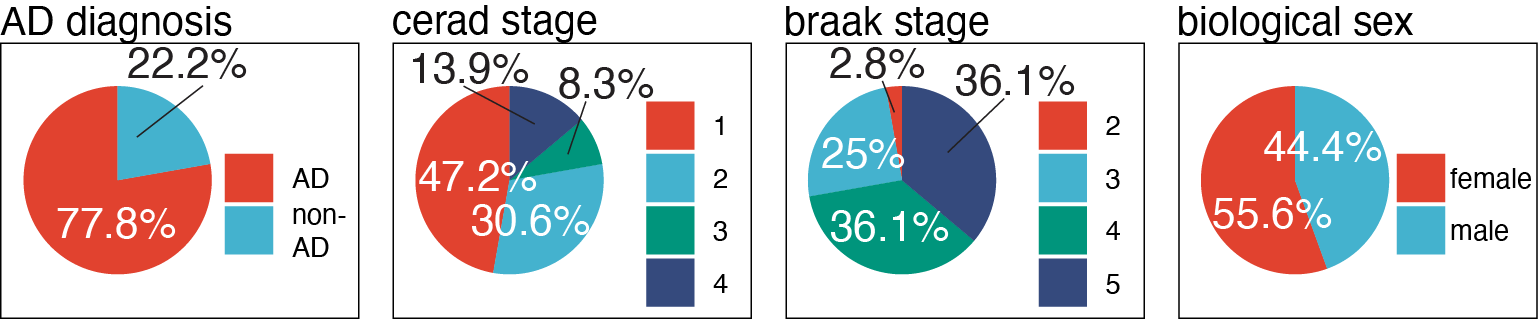
\includegraphics[width=\textwidth]{./main_plots/pie_charts.png}        
        \end{subfigure}
        \begin{subfigure}[t]{.45\textwidth}
            \caption{}
            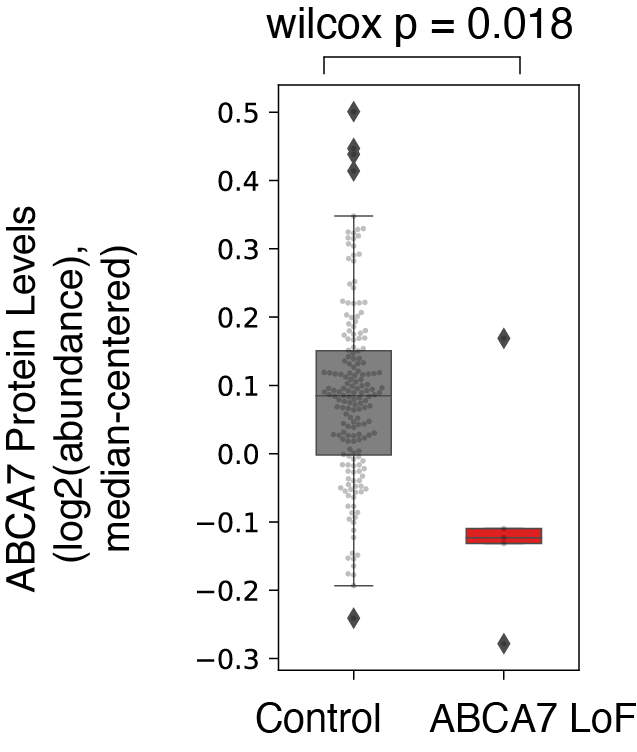
\includegraphics[width=\textwidth]{./main_plots/abca7_protein_levels.png}        
        \end{subfigure}
        \begin{subfigure}[t]{.5\textwidth}
            \caption{}
            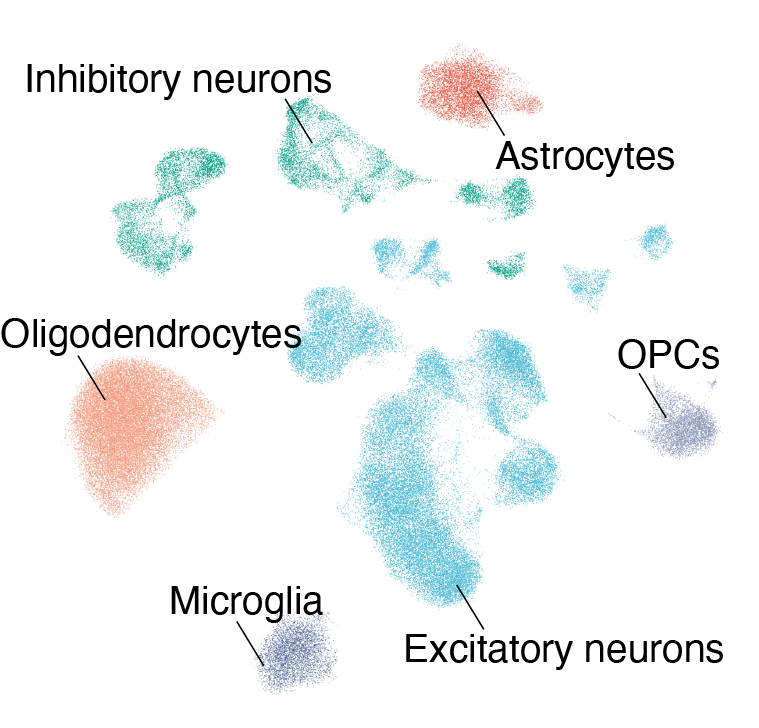
\includegraphics[width=\textwidth]{./main_plots/cell_projection.png}        
        \end{subfigure}
    \\[-3ex] 
    \end{subfigure}
    \begin{subfigure}[t]{0.5\textwidth}
        \caption{}
        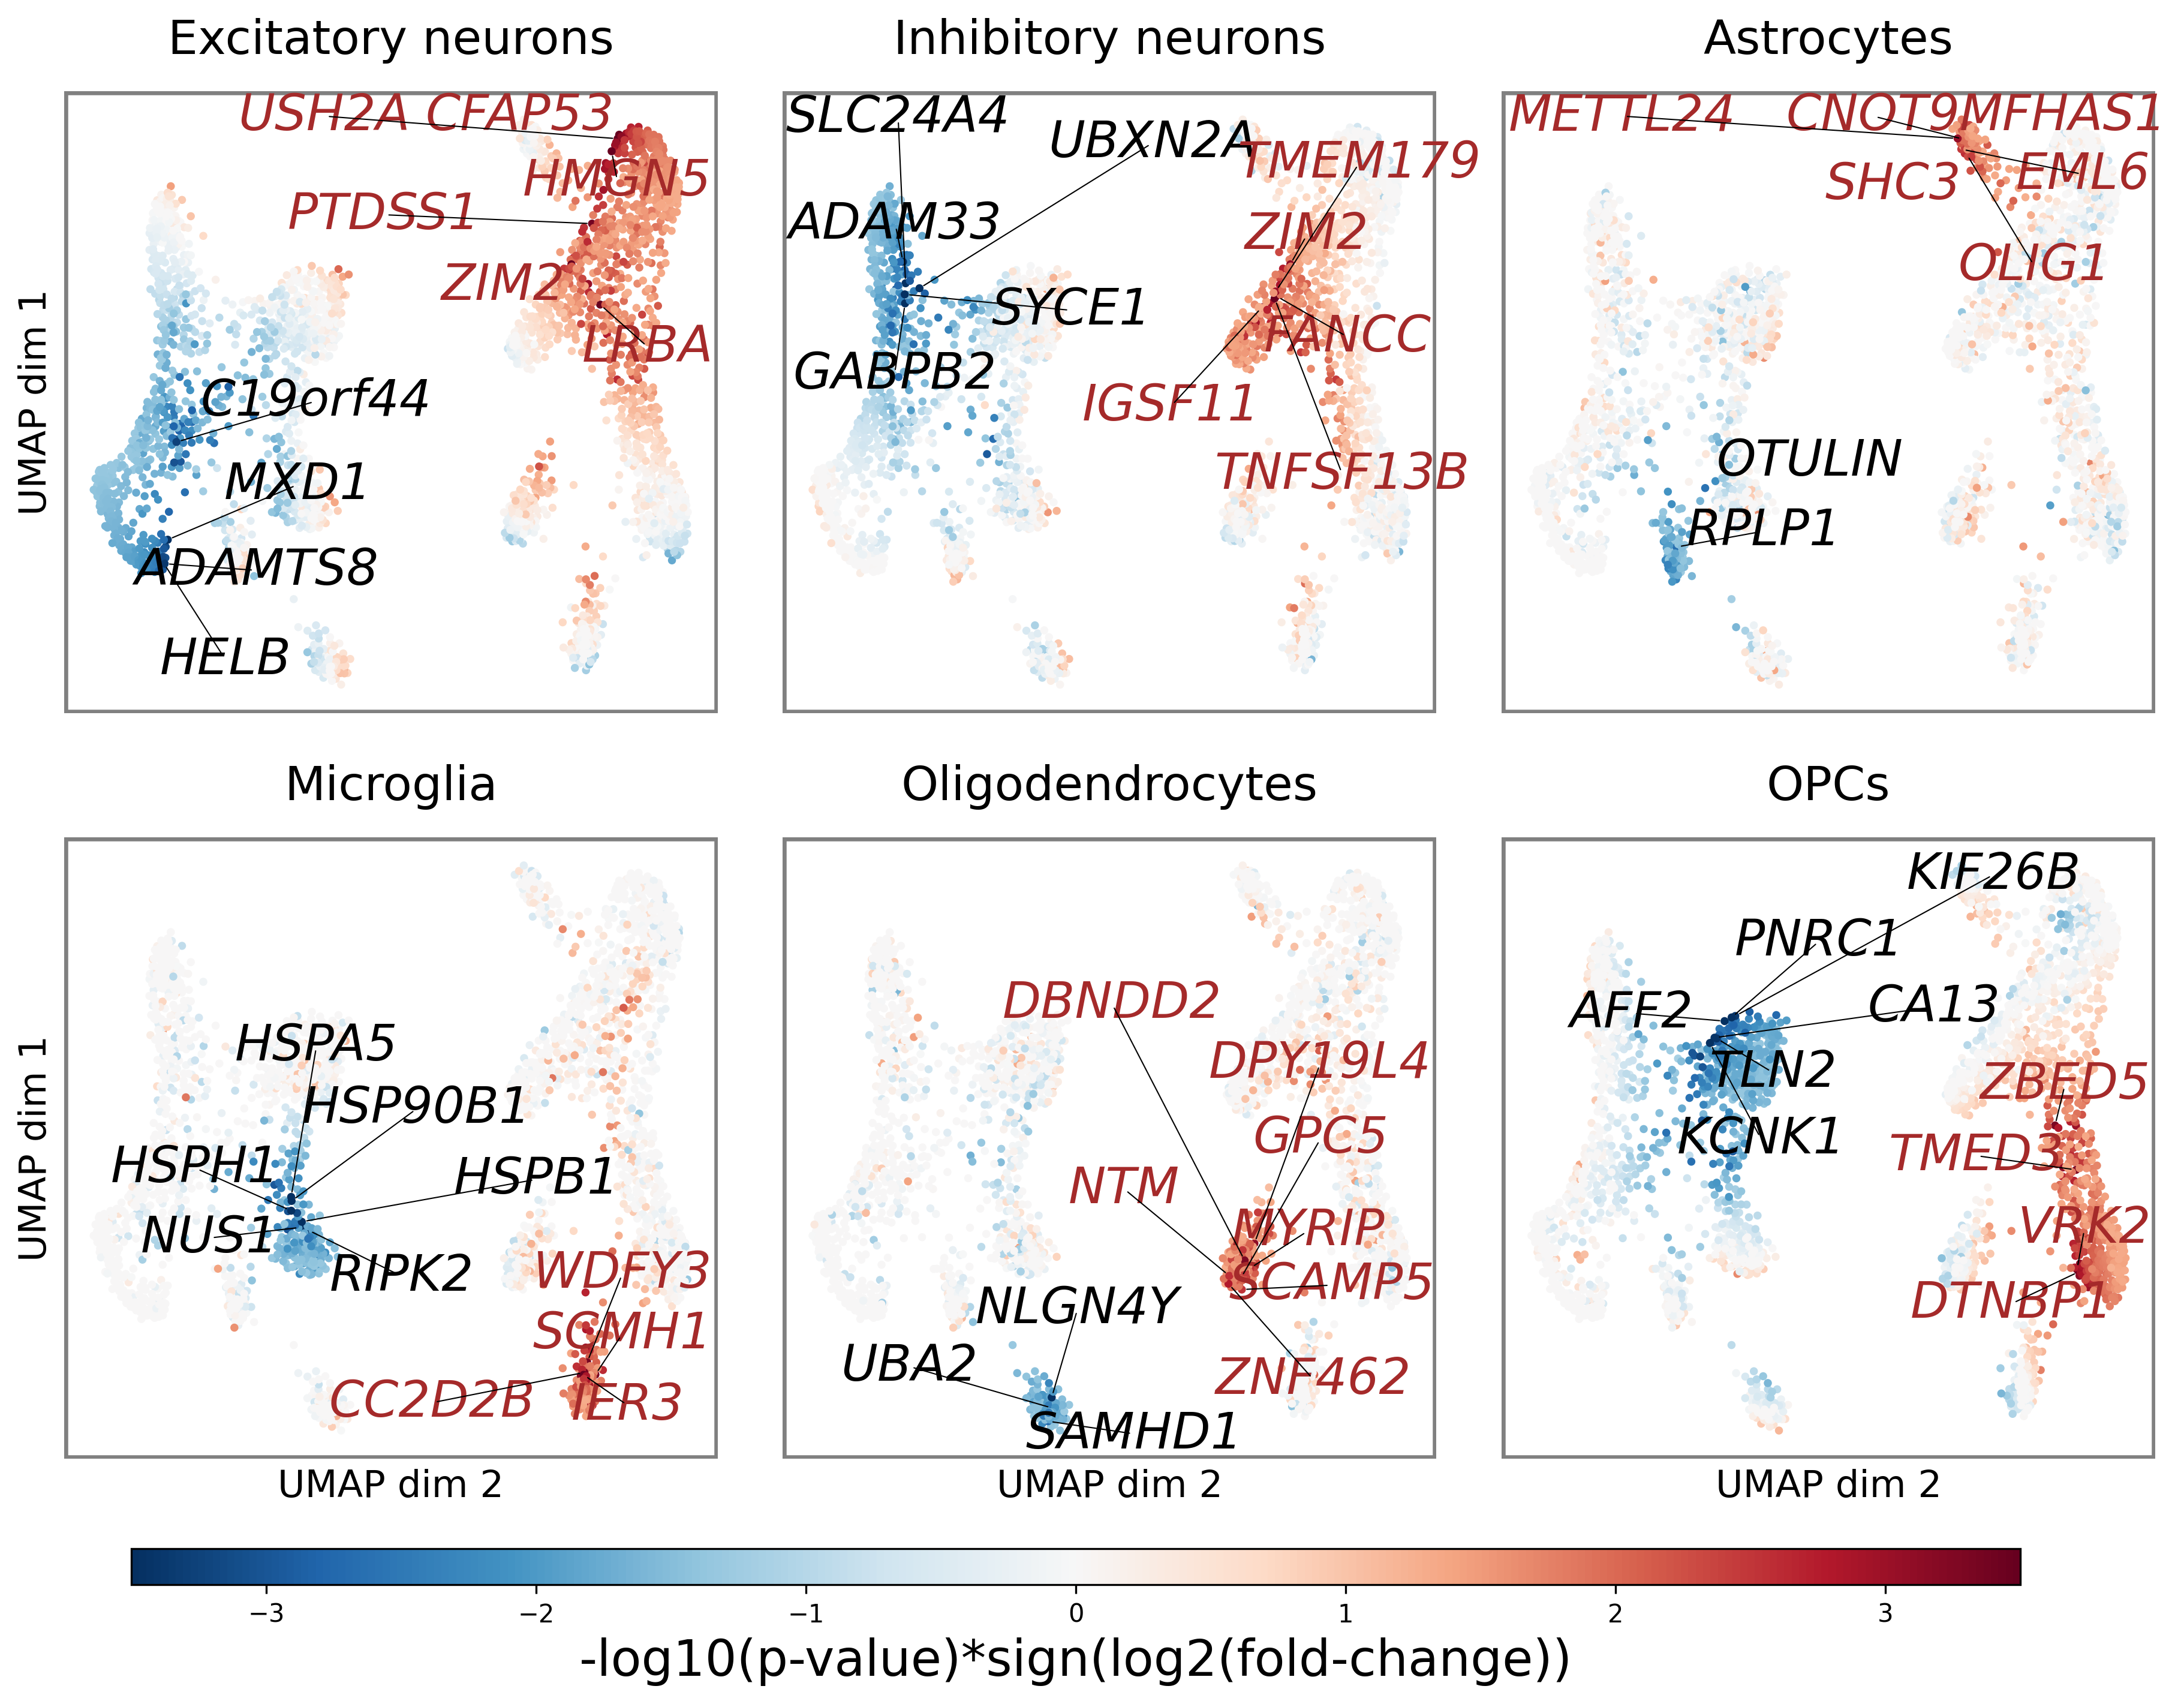
\includegraphics[width=\textwidth]{./main_plots/umap_projection_top_genes.png}        
    \end{subfigure}
    \begin{subfigure}[t]{\textwidth}
        \caption{}
        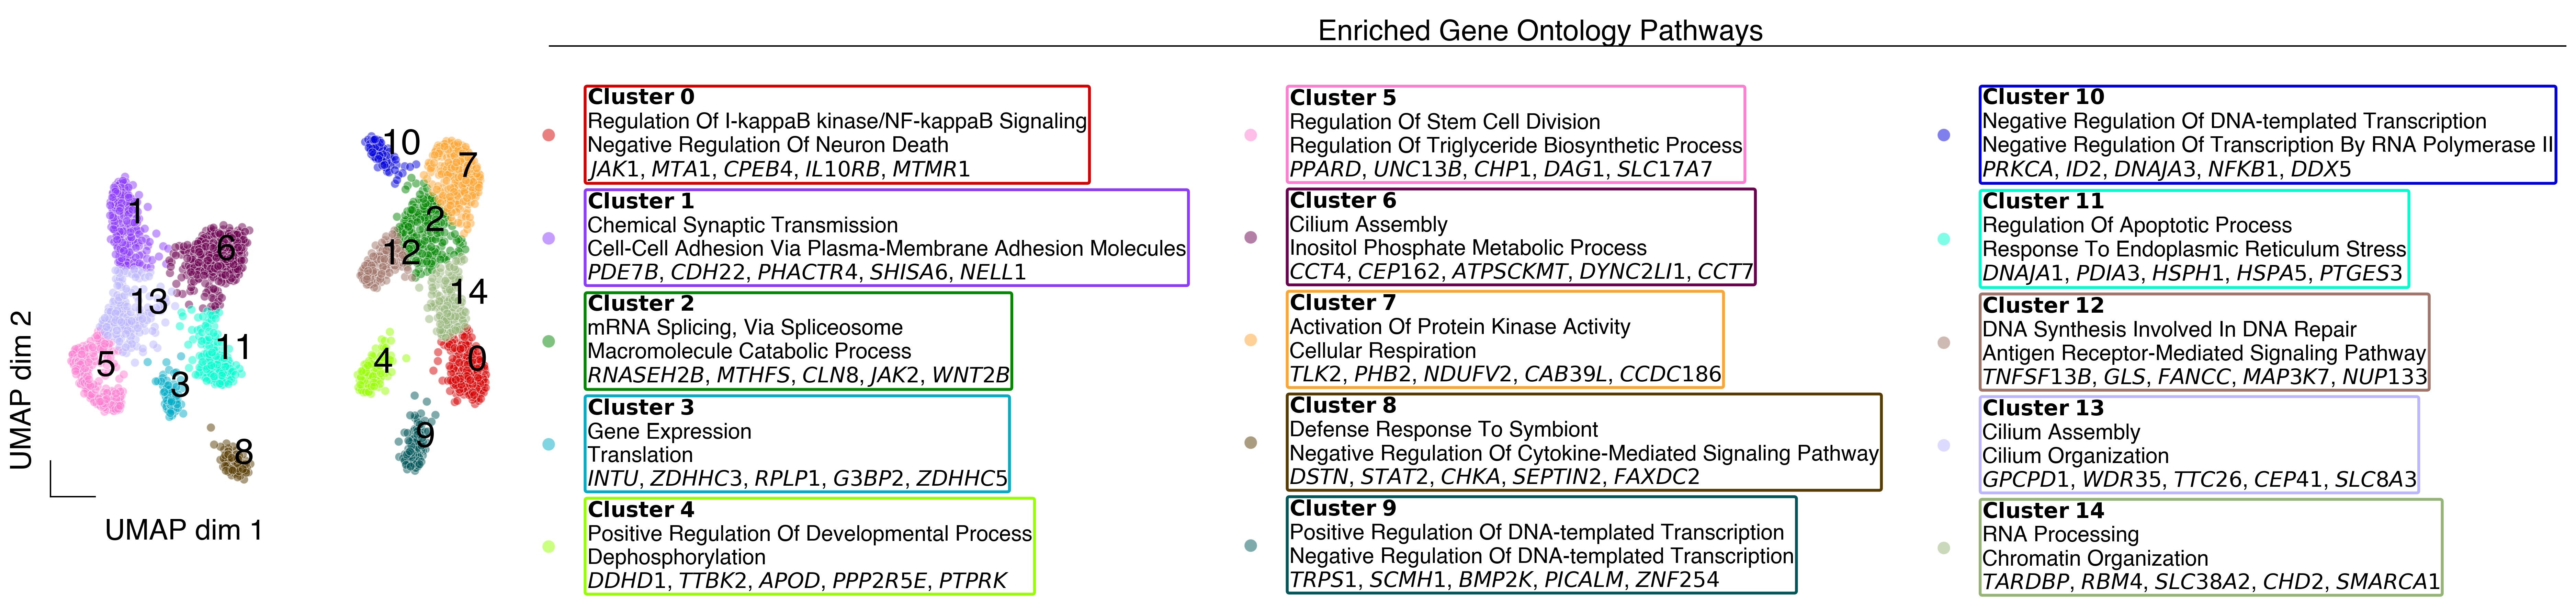
\includegraphics[width=\textwidth]{./main_plots/clusters_umap.png}        
    \end{subfigure}
    \\[-2ex] 
    \begin{subfigure}[t]{\textwidth}
        \caption{}
        
\includegraphics[width=\textwidth]{./main_plots/clusters_bars.png}        
    \end{subfigure}
    \caption{
        \textbf{Single-nuclear RNA-sequencing Atlas of Human Post-mortem Prefrontal Cortex Reveals Cell Type-specific Gene Changes in ABCA7 LoF.}\\
        }
    \label{fig:main_atlas}
\end{figure}
\begin{itemize}
\item[\textbf{(A)}] Overview of ABCA7 gene structure with the location of variants represented in this study (average minor allele frequency for depicted variants is < 1\%). Exons are depicted as black rectangles, and introns as black lines. The pie chart indicates the frequency of ABCA7 PTC-variant-carriers within the ROSMAP cohort. 
\item[\textbf{(B)}] Overview of human cohort for snRNA-seq (Created with BioRender.com). 
\item[\textbf{(C)}] Overview of snRNA-seq cohort metadata for 32 individuals. 
\item[\textbf{(D)}] ABCA7 protein levels (log2(abundance)) from post-mortem human prefrontal cortex in all available controls ($N=180$) vs. ABCA7 LoF carriers ($N=5$). P-value computed by Wilcoxon rank sum test. Boxes indicate per-condition dataset quartiles, and whiskers extend to the most extreme data points not considered outliers (i.e., within 1.5 times the interquartile range from the first or third quartile). 
\item[\textbf{(E)}] 2D UMAP projection of per-cell gene expression values and their transcriptionally defined cell type. 
\item[\textbf{(F)}] 2D UMAP projection of ABCA7 LoF gene perturbation scores ($S = -\log_{10}(\text{p-value}) \times \text{sign}(\log_2(\text{fold change}))$); Red = $S>1.3$, Blue = $S<-1.3$; Point size indicates $|S|$). Up to top 20 genes by $|S|$ are labeled. 
\item[\textbf{(G)}] Genes in 2D UMAP space colored by cluster assignment (Gaussian mixture model; see Methods) with per-cluster pathway enrichments shown (GO BP, hypergeometric enrichment, $p<0.01$). 
\item[\textbf{(H)}] Cell type-specific gene cluster scores ($SC = \text{mean}(S_i)$, for genes $i$ in cluster $c$). * indicates permutation FDR-adjusted p-value $< 0.01$ and $|SC| > 0.25$.
\end{itemize}
\clearpage

\begin{figure}[H]
    \begin{subfigure}[t]{0.45\textwidth}
        \begin{subfigure}[t]{0.49\textwidth}
            \caption{}
            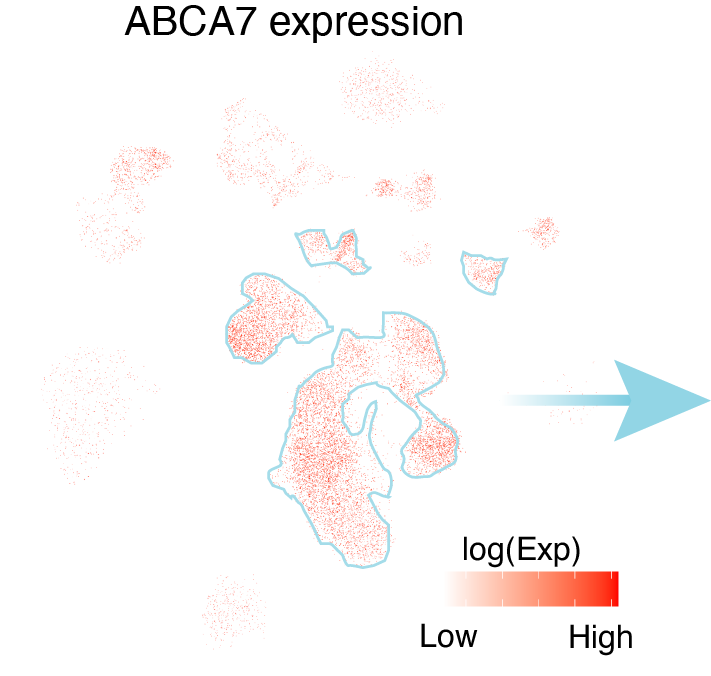
\includegraphics[width=\textwidth]{./main_plots/cell_projection_abca7_expression.png}        
        \end{subfigure}
        \begin{subfigure}[t]{0.49\textwidth}
            \caption{}
            \includegraphics[width=\textwidth]{./main_plots/pm_kl_network_network.pdf}        
        \end{subfigure}
        \begin{subfigure}[t]{\textwidth}
            \caption{}
            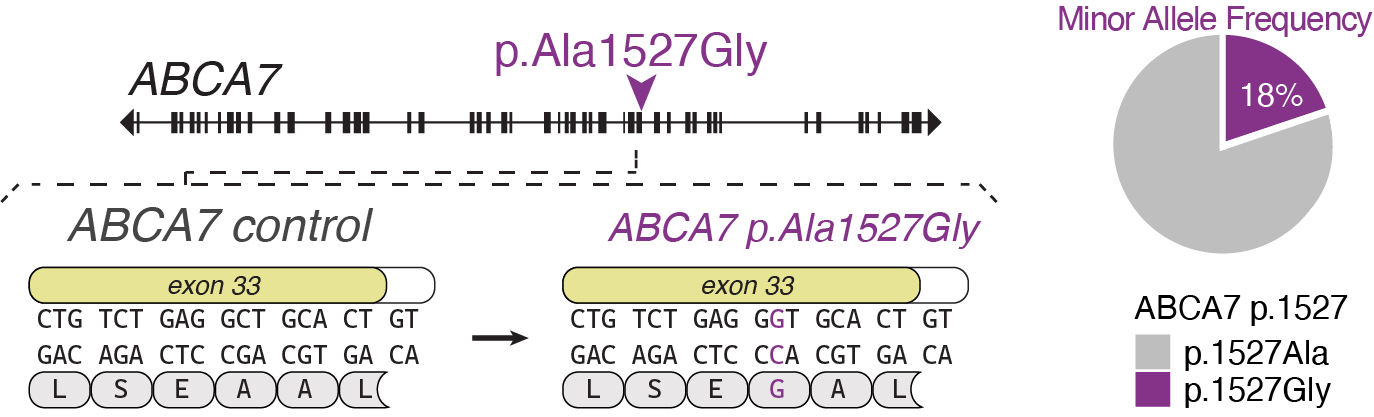
\includegraphics[width=\textwidth]{./main_plots/common_variant_cartoon.png}        
        \end{subfigure}
    \end{subfigure}
    \begin{subfigure}[t]{0.45\textwidth}
        \caption{}
        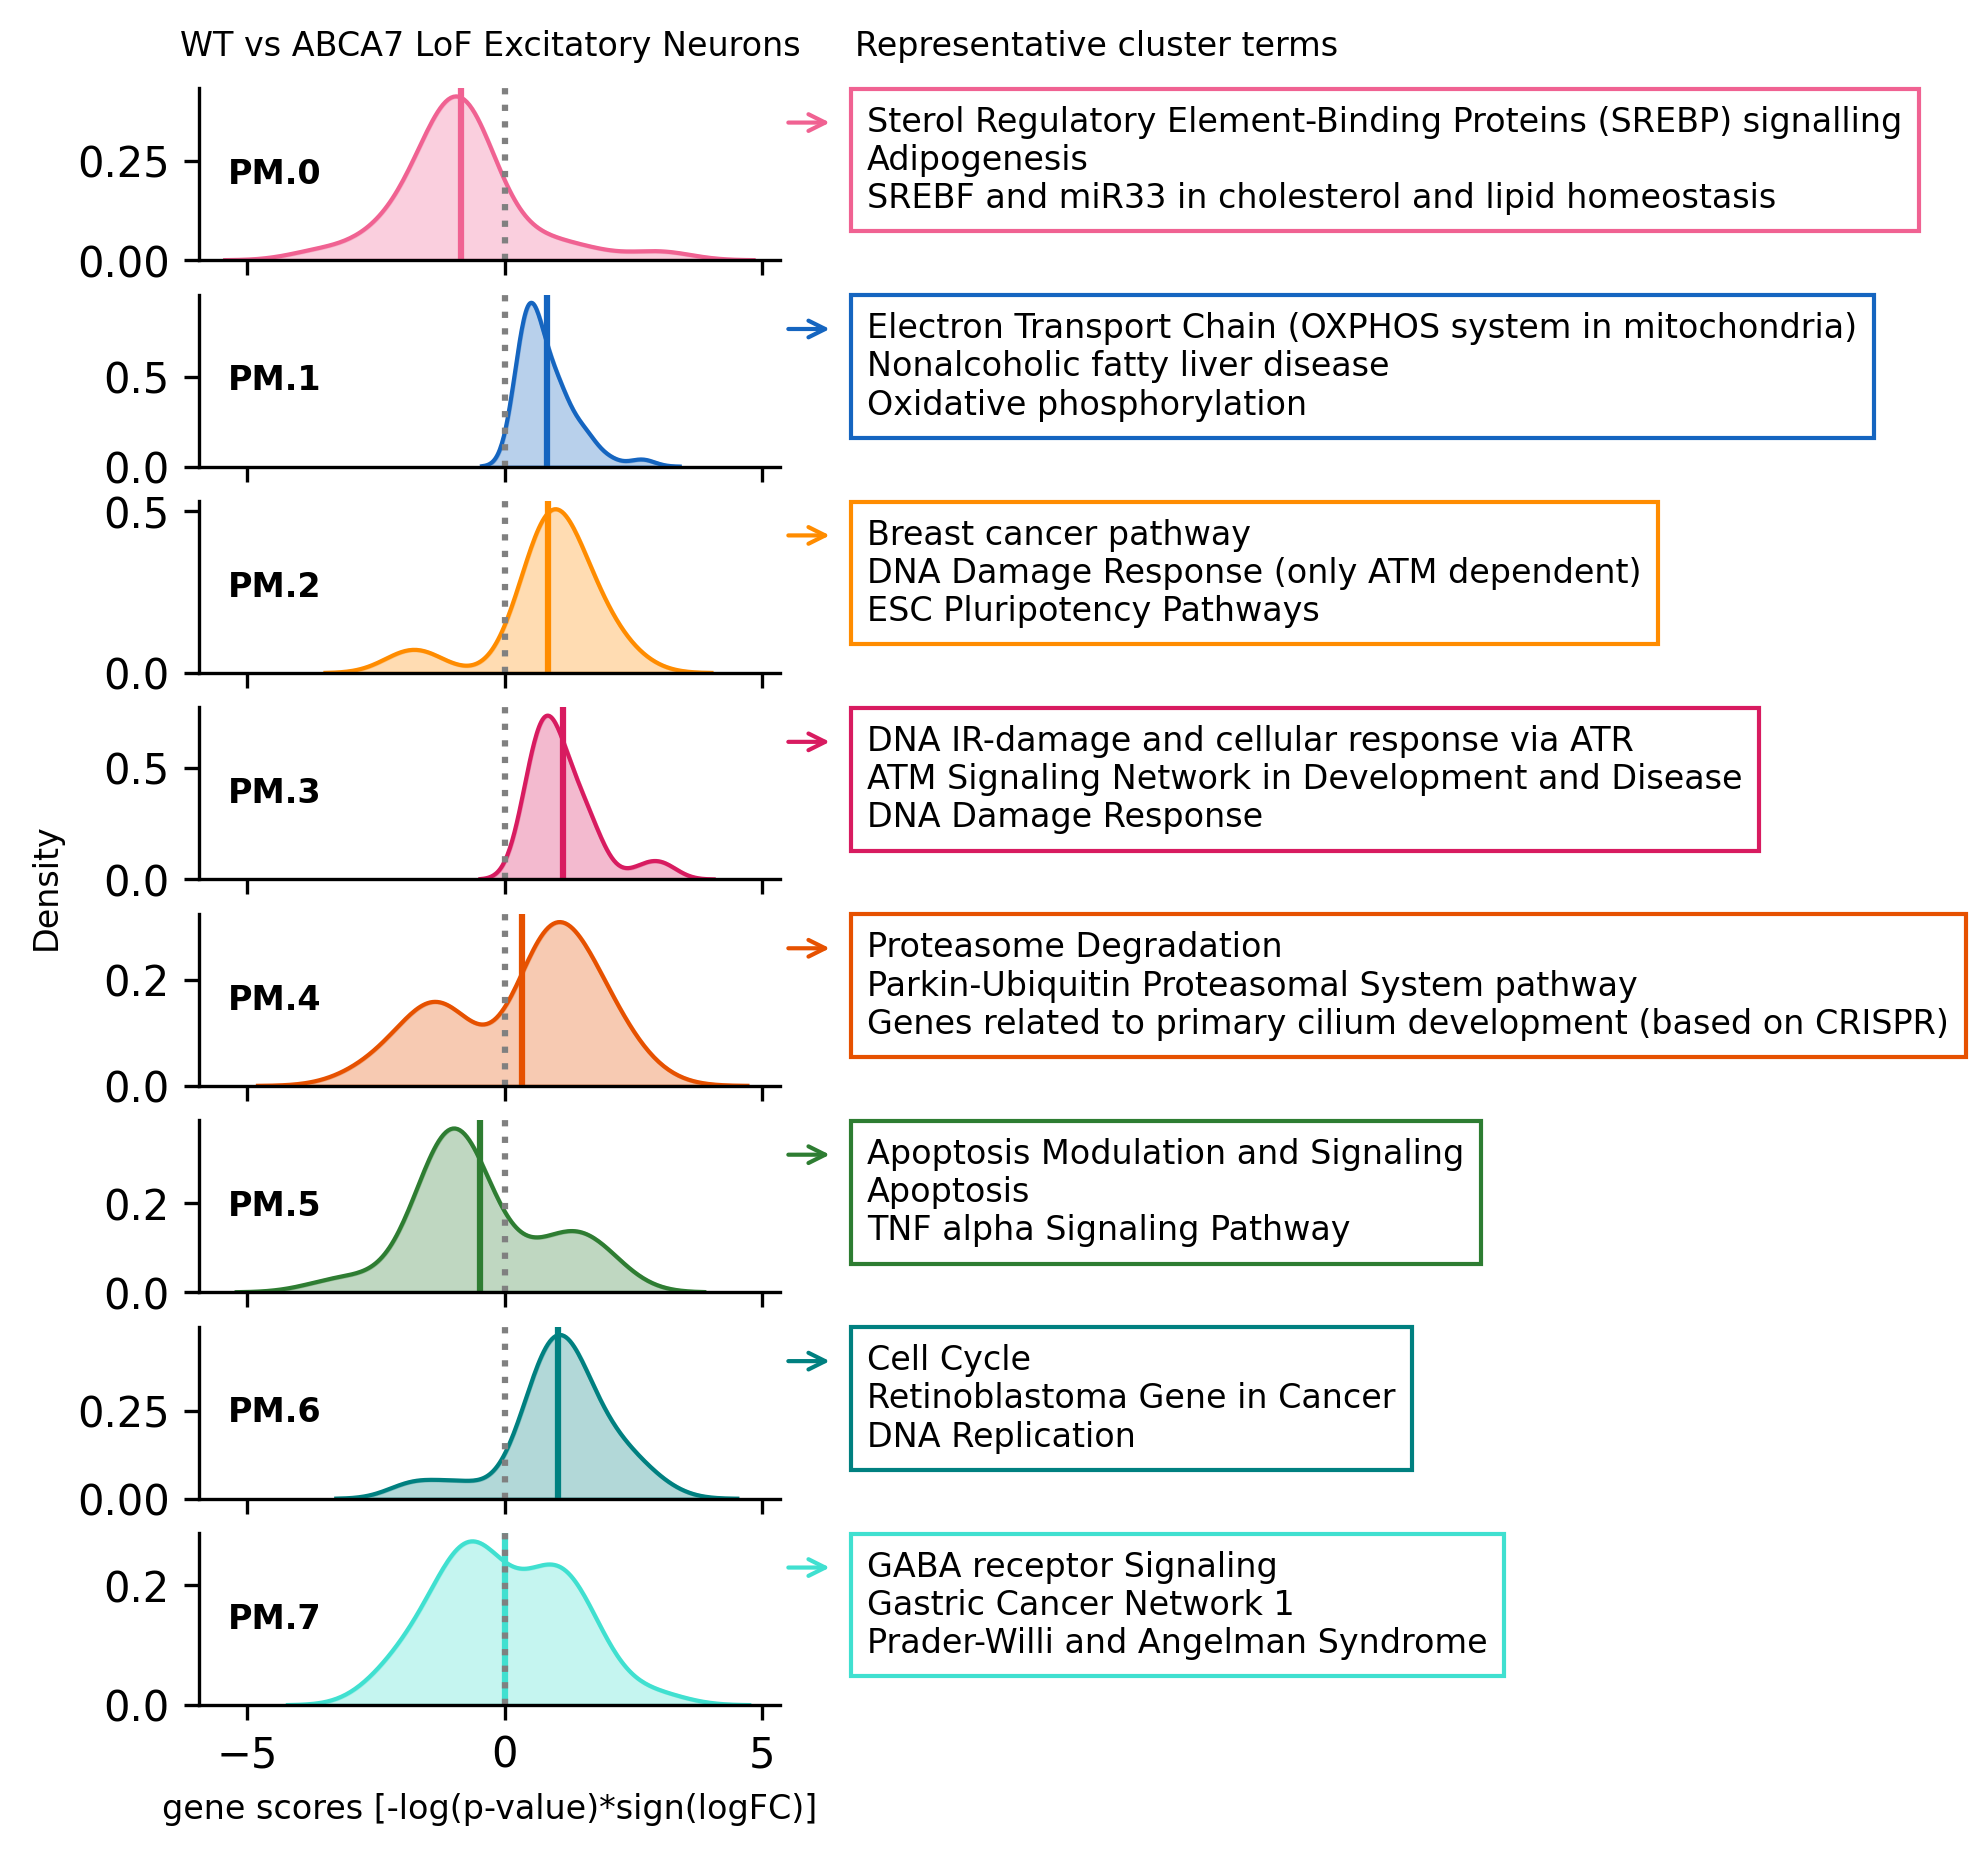
\includegraphics[width=\textwidth]{./main_plots/kl_densities.png}        
    \end{subfigure}
    \begin{subfigure}[t]{0.3\textwidth}
        \caption{}
        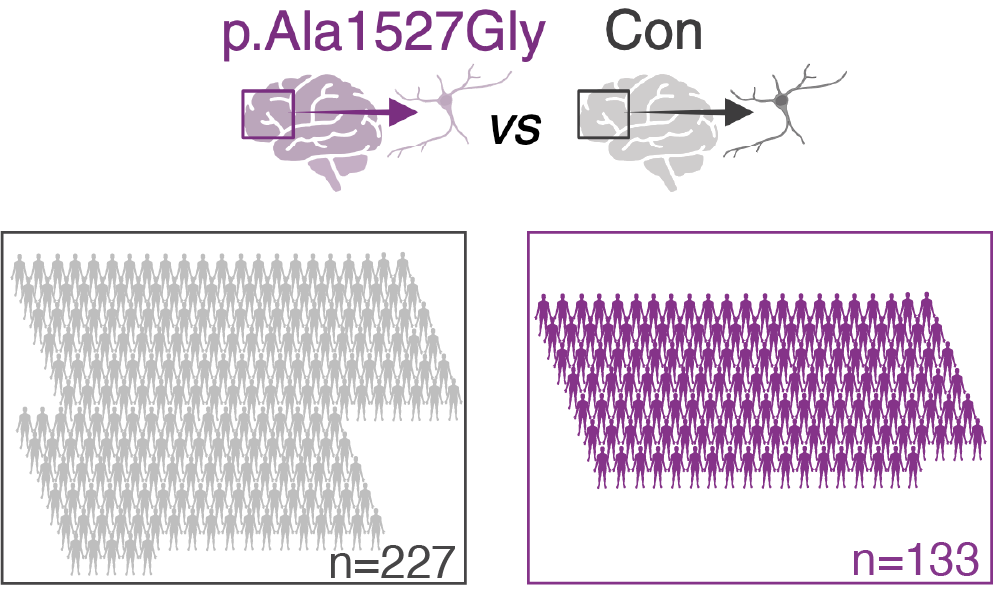
\includegraphics[width=\textwidth]{./main_plots/common_var_cohort_cartoon.png}        
    \end{subfigure}
    \hspace{0.01\textwidth} % Adjust this value as needed
    \begin{subfigure}[t]{0.225\textwidth}
        \caption{}
        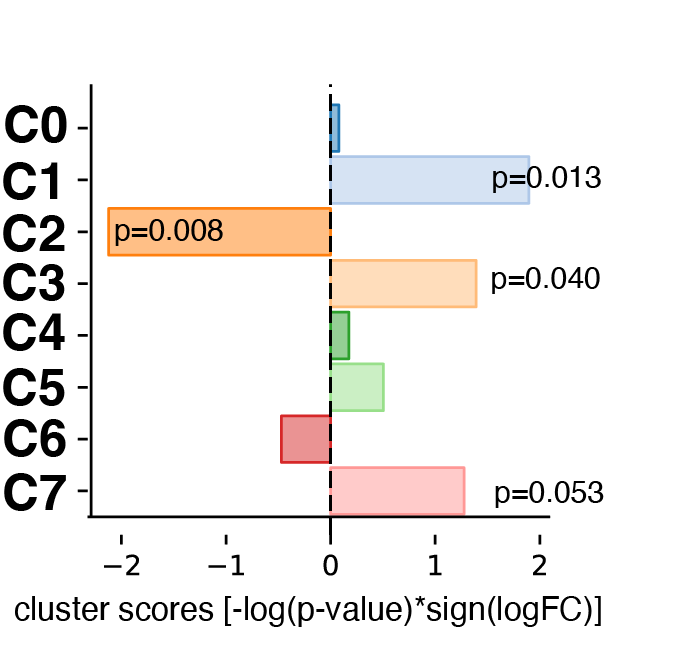
\includegraphics[width=\textwidth]{./main_plots/variant_path_scores.png}        
    \end{subfigure}
    \begin{subfigure}[t]{0.45\textwidth}
        \caption{}
        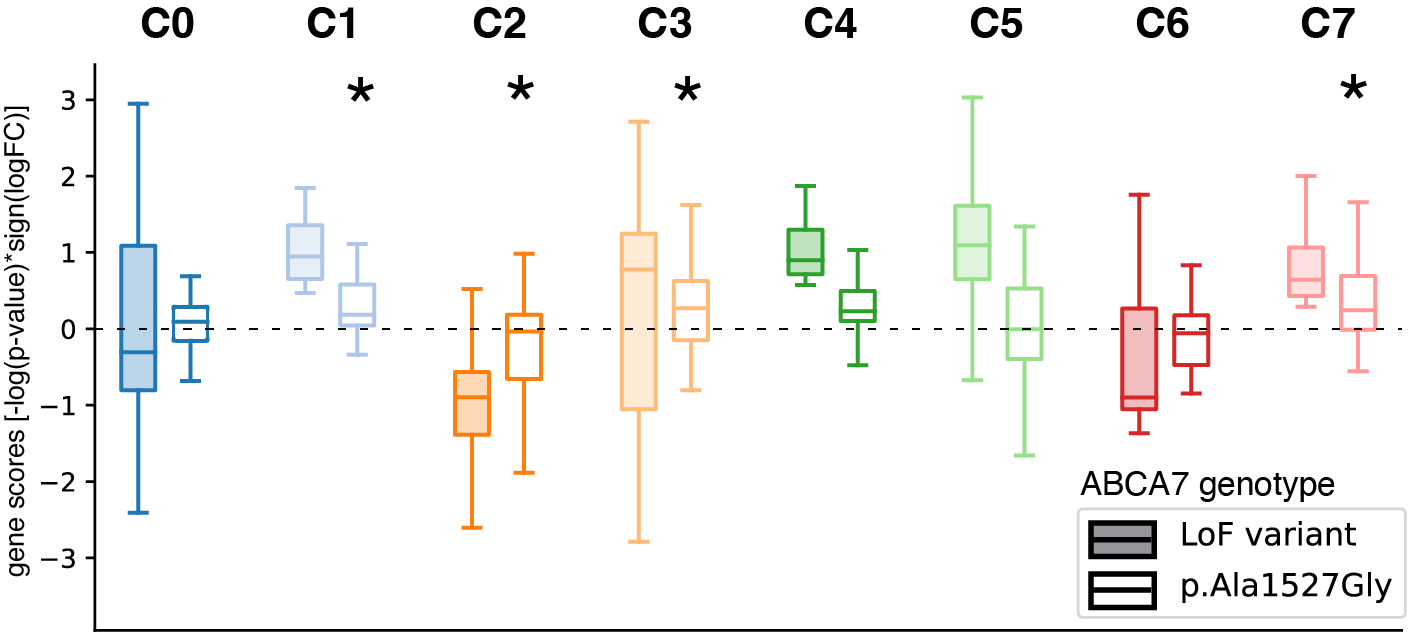
\includegraphics[width=\textwidth]{./main_plots/common_var_distributions.png}        
    \end{subfigure}
    \begin{subfigure}[t]{0.3\textwidth}
        \caption{}
        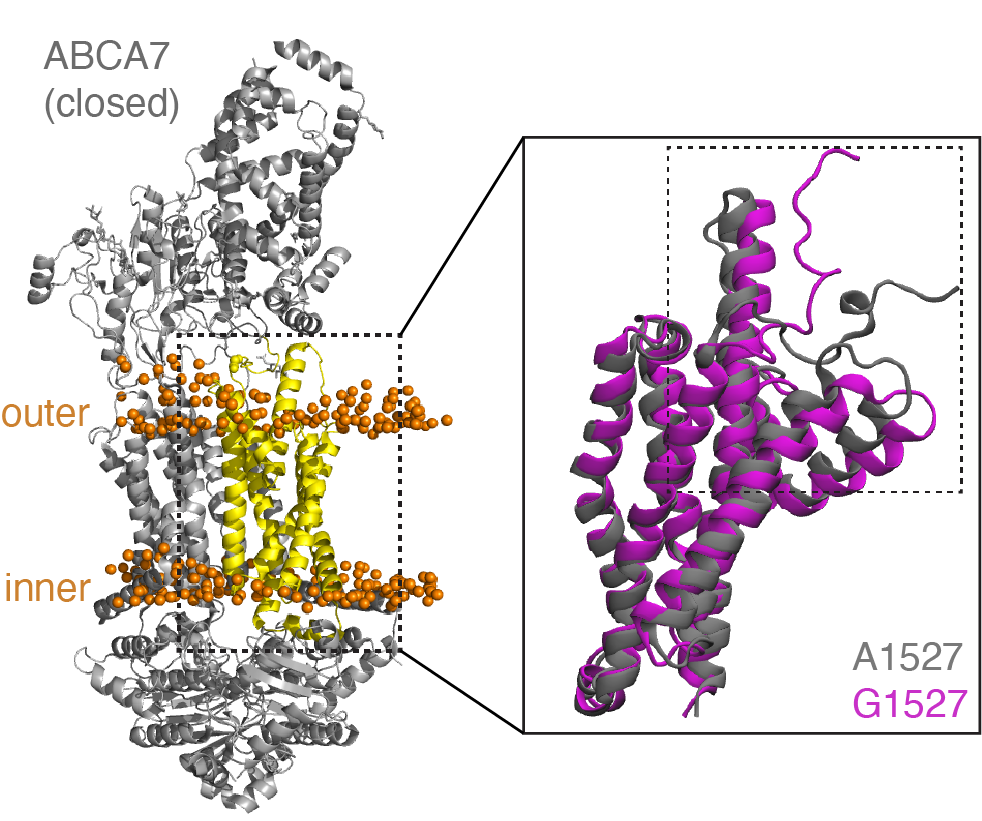
\includegraphics[width=\textwidth]{./main_plots/abca7_structure_with_inset.png}        
    \end{subfigure}
    \begin{subfigure}[t]{0.165\textwidth}
        \caption{}
        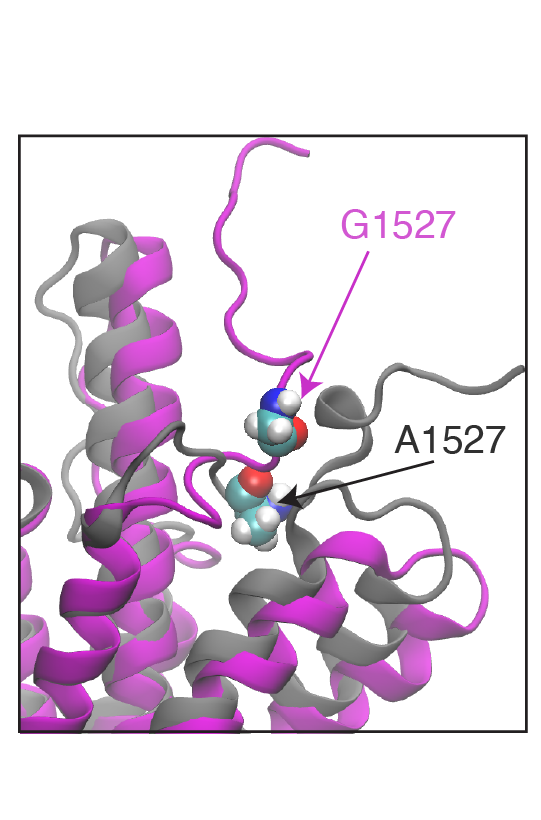
\includegraphics[width=\textwidth]{./main_plots/abca7_inset_only.png}        
    \end{subfigure}
    \hspace{0.01\textwidth} % Adjust this value as needed
    \begin{subfigure}[t]{0.32\textwidth}
        \caption{}
        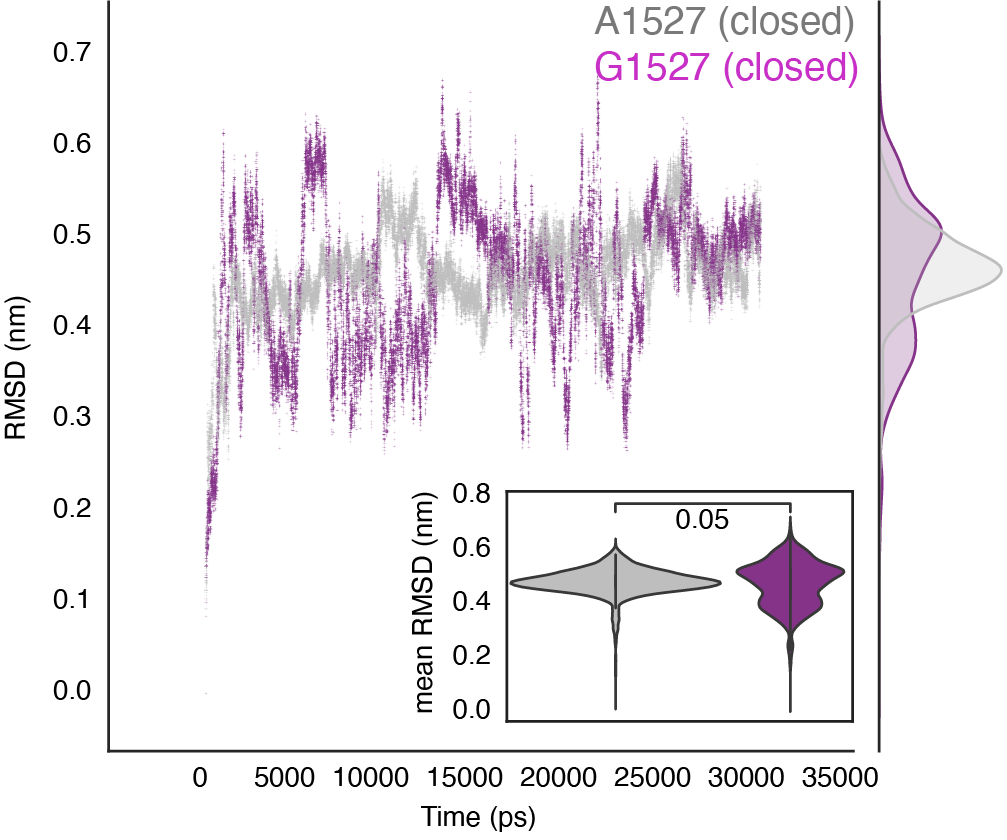
\includegraphics[width=\textwidth]{./main_plots/variant_dynamics.png}        
    \end{subfigure}
    \begin{subfigure}[t]{0.16\textwidth}
        \caption{}
        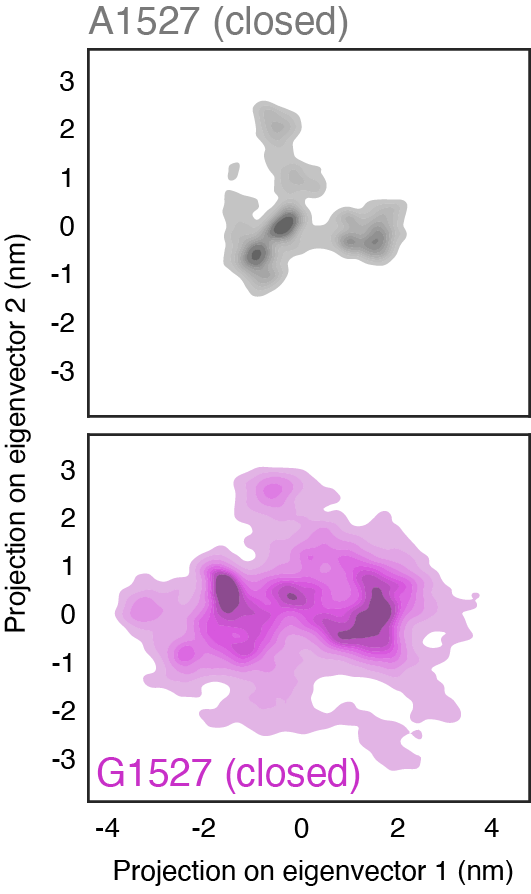
\includegraphics[width=\textwidth]{./main_plots/variant_projection_closed.png}        
    \end{subfigure}
    \caption{
        \textbf{Transcriptional Perturbations in Excitatory Neurons in ABCA7 LoF and ABCA7 p.Ala1527Gly Variant Carriers.}\\
    }
    \label{fig:main_neurons}
\end{figure}
\begin{itemize}
    \item[\textbf{(A)}] 2D UMAP projection of individual cells colored by log(Exp), where Exp represents log-normalized ABCA7 expression values.
    \item[\textbf{(B)}] Kernighan-Lin (K/L) clustering on leading edge genes from pathways perturbed in ABCA7 LoF excitatory neurons, where $p<0.05$. Colors indicate distinct K/L gene clusters, which are numbered from 0 to 7.
    \item[\textbf{(C)}] Left: Gaussian kernel density estimate plots of gene scores $S$ for genes belonging to a given gene cluster. $S>0$ indicates upregulation in ABCA7 LoF. Solid lines indicate distribution means. Right: Representative pathways that annotate the largest number of genes within a cluster (i.e., with the highest intra-cluster connectivity) shown per-cluster. 
    \item[\textbf{(D)}] Schematic indicating the genomic location of the p.Ala1527Gly codon change. A purple arrow indicates the location of the missense variant in the ABCA7 gene. Minor allele frequency shown to the right. 
    \item[\textbf{(E)}] Overview of snRNA-seq cohort of ABCA7 p.Ala1527Gly carriers (homozygous and heterozygous) vs. control non-carriers (minor allele frequency approx. 18\%).
    \item[\textbf{(F)}] Perturbation of ABCA7 LoF-associated gene clusters from (B-D) in excitatory neurons of p.Ala1527Gly variant-carriers vs. non-carrier controls, computed by FGSEA. Top $p$-values ($p<0.1$) are indicated. $S>0$ indicates upregulation in carriers.
    \item[\textbf{(G)}] Distributions of gene scores $S$ for genes belonging to a given gene cluster for ABCA7 p.Ala1527Gly (no fill) or ABCA7 LoF-variants (solid fill). $S>0$ indicates upregulation in ABCA7 variant. * indicates FGSEA $p$-value<0.1 from (G). Boxes indicate per-condition dataset quartiles, and whiskers extend to the most extreme data points not considered outliers (i.e., within 1.5 times the interquartile range from the first or third quartile).
    \item[\textbf{(H)}] Closed conformation ABCA7 protein structure. ABCA7 domain between residues 1517 and 1756 used for simulations is shown in yellow. Lipid bilayer shown in orange. Expanded yellow domain shown in inset, with A1527 variant (light grey) and G1527 variant (purple).
    \item[\textbf{(I)}] Expanded inset from H with residues of interest rendered.
    \item[\textbf{(J)}] Root mean squared deviations of closed conformation domains from I with A1527 (light grey) or G1527 (purple) under simulation. Structural deviations over time were computed with respect to reference closed conformation from I. Violin plot inset indicates average $C_\alpha$ atom positional fluctuations over time.
    \item[\textbf{(K)}] Projection of $C_\alpha$ atom positional fluctuations under simulation onto the first two principal components, for closed conformation domain from J with A1527 (top, light grey) or G1527 (bottom, purple). 
\end{itemize}
\clearpage

\begin{figure}[H]
    \begin{subfigure}[t]{.3\textwidth}
        \caption{}
        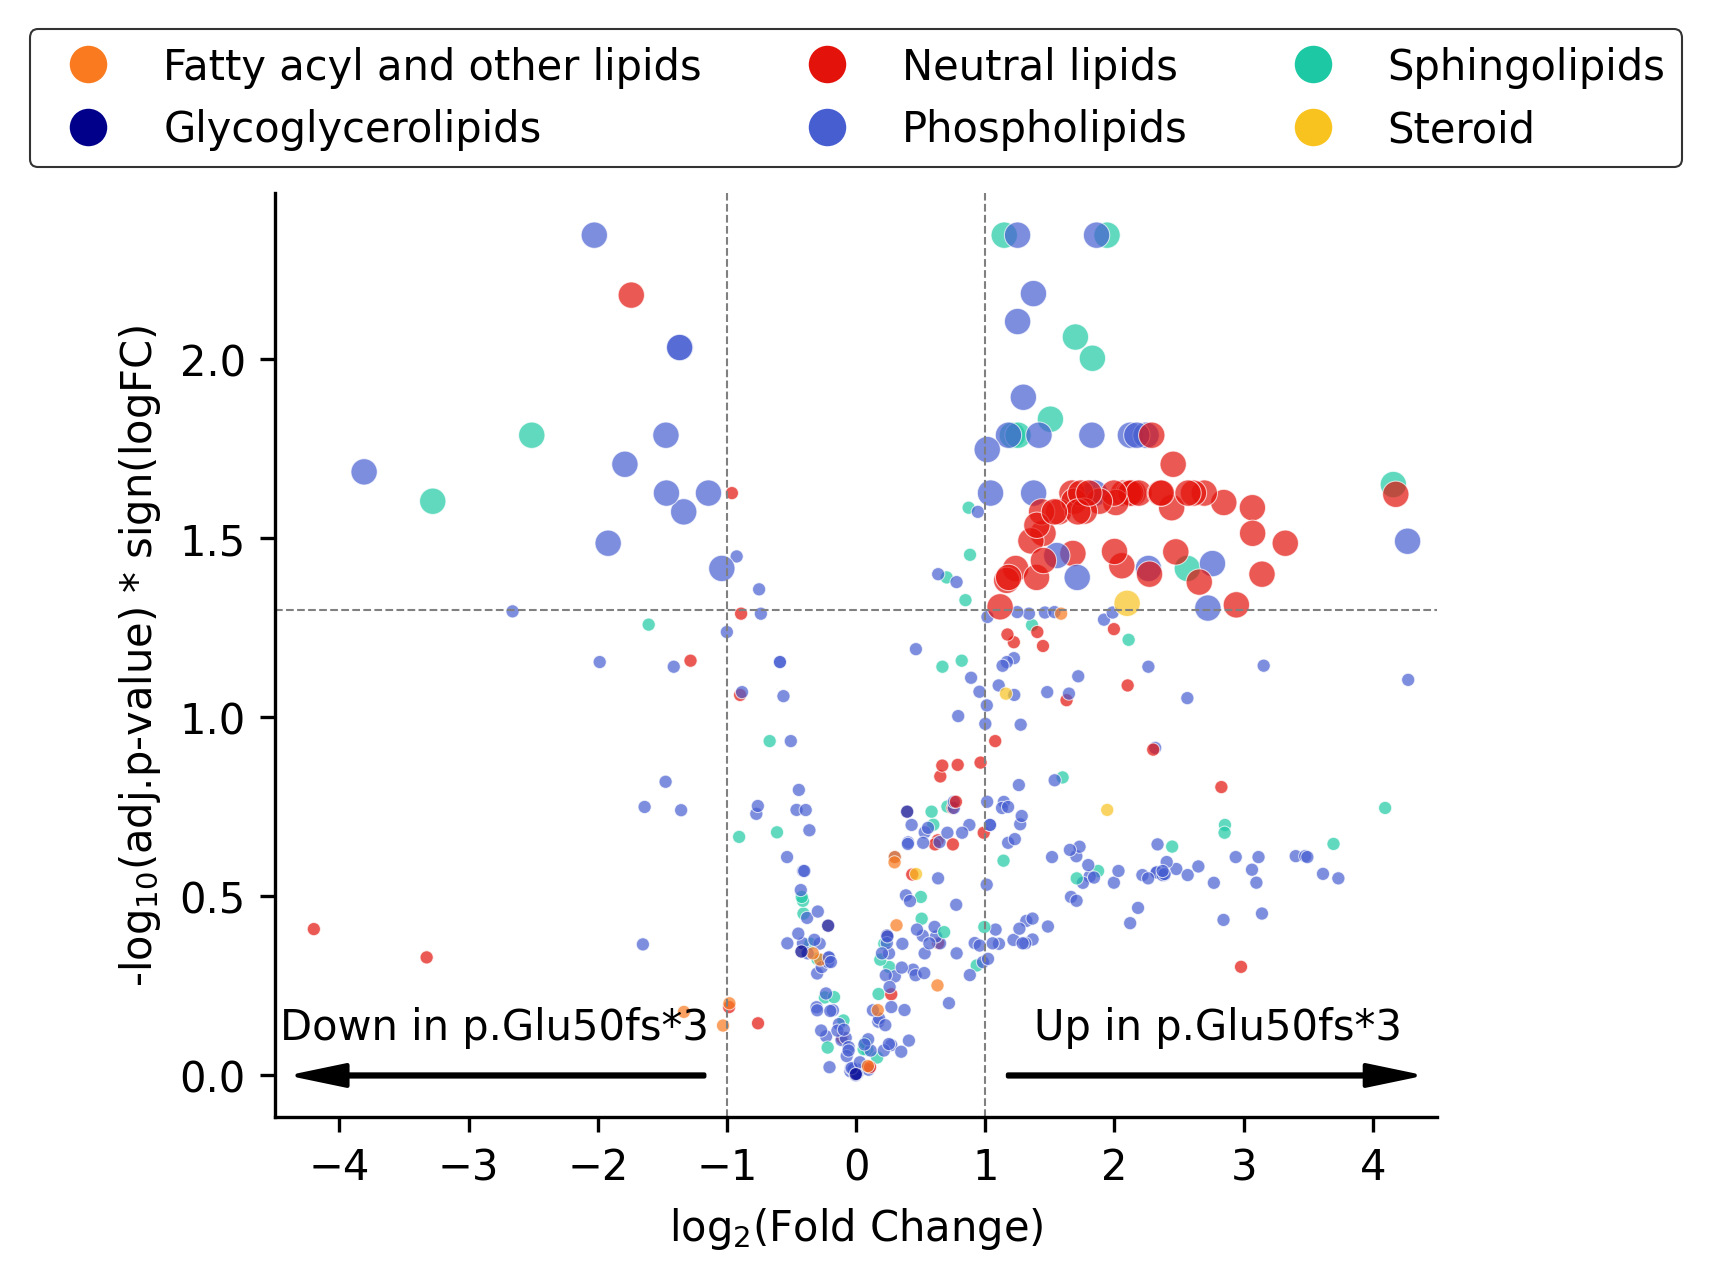
\includegraphics[width=\textwidth]{../paper/main_plots/iN_lipids_overview.png}        
    \end{subfigure} 
    \begin{subfigure}[t]{.3\textwidth}
        \caption{}
        \includegraphics[width=\textwidth]{../paper/main_plots/lipids_table.png}        
    \end{subfigure} 
    \begin{subfigure}[t]{.3\textwidth}
        \caption{}
        \includegraphics[width=\textwidth]{../paper/main_plots/tg_carbons.png}        
    \end{subfigure} 
    \begin{subfigure}[t]{.3\textwidth}
        \caption{}
        \includegraphics[width=\textwidth]{../paper/main_plots/G2_PC_volcano_sat.png}        
    \end{subfigure} 
    \begin{subfigure}[t]{.3\textwidth}
        \caption{}
        \includegraphics[width=\textwidth]{../paper/main_plots/G2_PC_volcano_unsat.png}        
    \end{subfigure} 
    \begin{subfigure}[t]{.3\textwidth}
        \caption{}
        \includegraphics[width=\textwidth]{../paper/main_plots/pc_unsat.png}        
    \end{subfigure} 
    \begin{subfigure}[t]{.3\textwidth}
        \caption{}
        \includegraphics[width=\textwidth]{../paper/main_plots/lipids_table_y622.png}        
    \end{subfigure}
    \begin{subfigure}[t]{.3\textwidth}
        \caption{}
        \includegraphics[width=\textwidth]{../paper/main_plots/Y622_PC_volcano_sat.png}        
    \end{subfigure} 
    \begin{subfigure}[t]{.3\textwidth}
        \caption{}
        \includegraphics[width=\textwidth]{../paper/main_plots/tg_carbons_y622.png}        
    \end{subfigure} 
    \begin{subfigure}[t]{.3\textwidth}
        \caption{}
        \includegraphics[width=\textwidth]{../paper/main_plots/pc_unsat_y622.png}        
    \end{subfigure} 
    \begin{subfigure}[t]{.2\textwidth}
        \caption{}
        \includegraphics[width=\textwidth]{../paper/extended_plots/g2_lpcat.png}        
    \end{subfigure} 
    \begin{subfigure}[t]{.2\textwidth}
        \caption{}
        \includegraphics[width=\textwidth]{../paper/extended_plots/y622_lpcat.png}        
    \end{subfigure} 
\end{figure}
\textbf{Extended Data Fig. 11}
\clearpage

\begin{figure}[H]
    % ROW 1
    
    \begin{subfigure}[t]{.24\textwidth}
        \begin{subfigure}[t]{\textwidth}
            \caption{}
            \includegraphics[width=\textwidth]{./main_plots/iN_gen2.png}        
            \includegraphics[width=\textwidth]{./extended_plots/variant_locations.png}        
            \includegraphics[width=\textwidth]{./main_plots/iN_rep_ims.png}        
        \end{subfigure} 
        \begin{subfigure}[t]{\textwidth}
            \caption{}
            \includegraphics[width=\textwidth]{./extended_plots/rna_correlation_both_lof_lines.png}        
        \end{subfigure} 
    \end{subfigure} 
    \hspace{.5cm}
    \begin{subfigure}[t]{.23\textwidth}
        \begin{subfigure}[t]{\textwidth}
            \caption{}
            \includegraphics[width=\textwidth]{./main_plots/y622_kl_clusters_network.pdf}        
        \end{subfigure}
        \begin{subfigure}[t]{\textwidth}
            \caption{}
            \centering
            \includegraphics[width=0.5\textwidth]{./main_plots/jaccard_cartoon.png}        
            \includegraphics[width=\textwidth]{./main_plots/jaccard_PM_pT622.png}        
        \end{subfigure}  
    \end{subfigure} 
    \hspace{.25cm}
    \begin{subfigure}[t]{.45\textwidth}
        \caption{}
        \includegraphics[width=\textwidth]{./main_plots/kl_densities_Tyr622.png}        
    \end{subfigure}  
    % Row 2
    \vspace{.25cm}
    \begin{subfigure}[t]{.25\textwidth}
        \begin{subfigure}[t]{\textwidth}
            \caption{}
            \includegraphics[width=\textwidth]{./main_plots/y622_mito_degs.png}        
        \end{subfigure}  
    \end{subfigure} 
    \begin{subfigure}[t]{.2\textwidth}
        \caption{}
            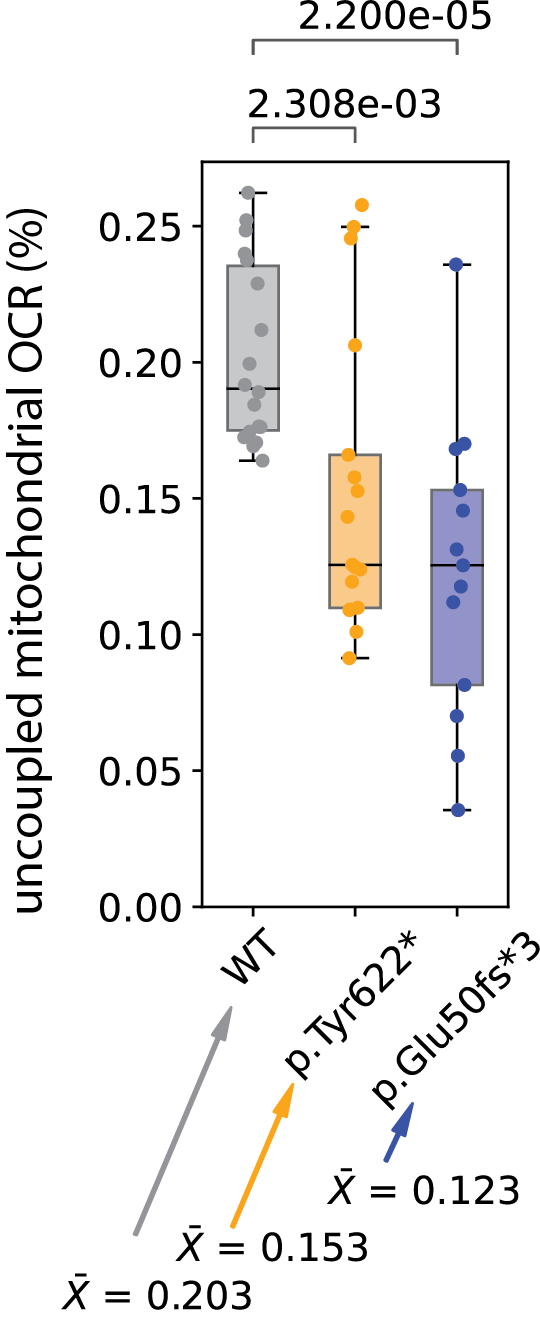
\includegraphics[width=\textwidth]{./main_plots/uncoupling.png}        
    \end{subfigure}   
    \begin{subfigure}[t]{.5\textwidth}
        \caption{}
        \includegraphics[width=\textwidth]{./extended_plots/mitohealth_y_g.png}        
    \end{subfigure}    
    % Row 3
    \begin{subfigure}[t]{.35\textwidth}
        \caption{}
        \includegraphics[width=\textwidth]{./main_plots/tmrm_main.png}        %tmrm_with_FCCP
    \end{subfigure}    
   % \hspace{1cm}
    \hspace{.25cm}
    \begin{subfigure}[t]{.35\textwidth}
        \caption{}
        \includegraphics[width=\textwidth]{./main_plots/cellrox_images.png}        
    \end{subfigure}  
    \hspace{.5cm}
    \begin{subfigure}[t]{.2\textwidth}
        \caption{}
        \includegraphics[width=\textwidth]{./main_plots/all_lipids_y622.png}        
    \end{subfigure}  
    \caption{
        \textbf{ABCA7 LoF Impairs Regulation of Mitochondrial Uncoupling in Neurons.}\\
    }
    \label{fig:main_mitochondrial}
\end{figure}
\begin{itemize}
\item[\textbf{(A)}] Schematic of iPSC-derived isogenic neuronal lines carrying ABCA7 LoF variants. The ABCA7 gene map highlights exons (black rectangles) and introns (black lines). CRISPR-Cas9 was used to introduce a premature termination codon in exon 3 (p.Glu50fs3, blue) or exon 15 (p.Tyr622, orange).\\
\item[\textbf{(B)}] Correlation of per-gene perturbation scores ($S = -\log_{10}(\text{p-value}) \times \text{sign}(\log_2(\text{fold change}))$) between p.Glu50fs3 vs. WT and p.Tyr622 vs. WT iNs.\\
\item[\textbf{(C)}] Kernighan-Lin (K/L) clustering of leading-edge genes from pathways perturbed in p.Tyr622* vs. WT iNs (p-adjusted < 0.05). Colors indicate distinct K/L gene clusters, which are assigned postmortem (PM) cluster labels if they significantly overlap with PM-identified clusters based on Jaccard analysis in (D). Otherwise, they are labeled with a 'T' prefix.\\
\item[\textbf{(D)}] Heatmap showing Jaccard index-based overlap between K/L clusters from p.Tyr622* vs. WT iNs and postmortem-identified clusters.\\
\item[\textbf{(E)}] Left: Gaussian kernel density estimate plots of gene scores $S$ for genes within each cluster ($S>0$ indicates upregulation in ABCA7 LoF). Solid lines represent distribution means. Right: Top representative pathways associated with the highest intra-cluster connectivity.\\
\item[\textbf{(F)}] Volcano plot of differentially expressed genes between p.Tyr622* and WT iNs, highlighting genes with mitochondrial localization.\\
\item[\textbf{(G)}] Uncoupled mitochondrial oxygen consumption rate (OCR) in WT vs. ABCA7 LoF iNs, measured by Seahorse assay. P-values computed via independent sample t-test. $N$ wells = 18 (WT), 17 (p.Tyr622*), 13 (p.Glu50fs*3) from two independent differentiation batches.\\
\item[\textbf{(H)}] Left: Quantification of mitochondrial membrane potential using HCS MitoHealth dye in neurons. P-values computed using a linear mixed-effects model on per-NeuN+ volume averages, with well-of-origin as a random effect. $N=8$ (WT), 11 (p.Tyr622*), 9 (p.Glu50fs*3), with ~3000 cells per condition from three independent differentiation batches. Right: Representative images showing NeuN+ cells and corresponding MitoHealth and Hoechst staining. MitoHealth images underwent percentile-based background subtraction and thresholding.\\
\item[\textbf{(I)}] Average TMRM fluorescence intensity in p.Tyr622* vs. WT iNs per mask (binarized TMRM signal based on the 75th percentile threshold) under baseline conditions and after FCCP treatment.\\
\item[\textbf{(J)}] Average CellROX fluorescence intensity in p.Tyr622* vs. WT iNs per mask (binarized CellROX signal based on the 75th percentile threshold).\\
\item[\textbf{(K)}] Volcano plot of differentially abundant lipid species between p.Tyr622* and WT iNs, colored by lipid class.
\end{itemize}
\clearpage

% \begin{figure}[H]
%    \includegraphics[width=\textwidth]{./main_plots/fig_5_temp.png}
    \begin{subfigure}[t]{.24\textwidth}
        \begin{subfigure}[t]{\textwidth}
            \caption{}
            \includegraphics[width=\textwidth]{./main_plots/all_lipids_choline_batch1.png}        
        \end{subfigure} 
        \begin{subfigure}[t]{\textwidth}
            \caption{}
            \vspace{-0.5cm}
            \centering
            \includegraphics[width=.8\textwidth]{./main_plots/rna_correlation_plot.png}        
        \end{subfigure}  
    \end{subfigure}  
    \hspace{.5cm}
    \begin{subfigure}[t]{.23\textwidth}
        \begin{subfigure}[t]{\textwidth}
            \caption{}
            \includegraphics[width=\textwidth]{./main_plots/Y622_choline_kl_network_network.pdf}        
        \end{subfigure}  
        \begin{subfigure}[t]{\textwidth}
            \caption{}
            \includegraphics[width=\textwidth]{./main_plots/jaccard_pT622_with_choline.png}        
        \end{subfigure} 
    \end{subfigure} 
    \hspace{.25cm}
    \begin{subfigure}[t]{.45\textwidth}
        \caption{}
        \includegraphics[width=\textwidth]{./main_plots/kl_densities_choline.png}        
    \end{subfigure}  
    \vspace{.05cm}
    \begin{subfigure}[t]{.24\textwidth}
        \caption{}
        \includegraphics[width=\textwidth]{./main_plots/choline_mito_degs.png}        
    \end{subfigure}  
    \hspace{.4cm} 
    \begin{subfigure}[t]{.17\textwidth}
        \caption{}
        \vspace{.3cm}
        \includegraphics[width=\textwidth]{./main_plots/pca_plot_y622_choline_metab.png}        
    \end{subfigure} 
    \hspace{.4cm}
    \begin{subfigure}[t]{.17\textwidth}
        \caption{}
        \vspace{.4cm}
        \includegraphics[width=\textwidth]{./main_plots/uncoupling_choline_quantification.png}        
    \end{subfigure}  
    \hspace{.4cm}  
    \begin{subfigure}[t]{.35\textwidth}
        \caption{}
        \vspace{-0.15cm}
        \includegraphics[width=\textwidth]{./main_plots/tmrm_choline.png}        
    \end{subfigure} 
   
    %%%% NEW ROW %%%%
    \begin{subfigure}[t]{.35\textwidth}
        \caption{}
        \includegraphics[width=\textwidth]{./main_plots/cellrox_images_choline.png}        
    \end{subfigure}
    \hspace{.4cm}
    \begin{subfigure}[t]{.4\textwidth}
        \caption{}
        \includegraphics[width=\textwidth]{./main_plots/abeta_elisa.png}        
    \end{subfigure}  
    \hspace{.4cm}
    \begin{subfigure}[t]{.15\textwidth}
        \caption{}
        \includegraphics[width=\textwidth]{./main_plots/temp.png}        
    \end{subfigure}  
    \caption{
        \textbf{CDP-choline Treatment Rescues ABCA7 LoF-Induced Disruptions in Neurons.}\\
    }
    \label{fig:main_choline}
\end{figure}
\begin{itemize}
    \item[\textbf{(A)}] Volcano plot showing differentially abundant lipid species between p.Tyr622* iNs with and without CDP-choline treatment, colored by lipid class. 
    \item[\textbf{(B)}] PCA plot of per-cell gene expression in p.Tyr622* iNs treated with CDP-choline or vehicle control. 
    \item[\textbf{(C)}] Kernighan-Lin (K/L) clustering of leading-edge genes from pathways perturbed in p.Tyr622* vs. WT iNs (p-adjusted < 0.05). Colors represent distinct K/L gene clusters, with clusters assigned p.Tyr622* vs. WT labels based on Jaccard analysis in 
    \item[\textbf{(D)}] Heatmap showing Jaccard index-based overlap between K/L clusters from p.Tyr622* vs. WT iNs and p.Tyr622* vs. CDP-choline iNs. 
    \item[\textbf{(E)}] Left: Gaussian kernel density estimate plots of gene scores (S) for genes in each cluster (S > 0 indicates upregulation in ABCA7 LoF). Solid lines show distribution means. Right: Representative pathways annotating the most genes within each cluster. 
    \item[\textbf{(F)}] Volcano plot of differentially expressed genes in p.Tyr622* iNs after CDP-choline treatment, highlighting those with mitochondrial protein localization. 
    \item[\textbf{(G)}] LC-MS metabolite profile projection onto the first two principal components. 
    \item[\textbf{(H)}] Relative mitochondrial uncoupling quantified by Seahorse oxygen consumption assay in 4-week-old p.Tyr622* iNs treated with CDP-choline or vehicle for 2 weeks. Uncoupling represents the proportion of basal oxygen consumption attributed to proton leak. P-values from independent t-tests, wells = 6 (p.Tyr622* + H2O), 8 (p.Tyr622* + CDP-choline). 
    \item[\textbf{(I)}] Average TMRM fluorescence intensity in p.Tyr622* iNs with or without CDP-choline, per mask (binarized TMRM signal based on the 75th percentile threshold) under baseline and FCCP treatment. 
    \item[\textbf{(J)}] Average CellROX fluorescence intensity in p.Tyr622* iNs with or without CDP-choline, per mask (binarized CellROX signal based on the 75th percentile threshold). 
    \item[\textbf{(K)}] Quantification of secreted Aβ levels in p.Tyr622* iNs with or without CDP-choline in cortical organoids. 
    \item[\textbf{(L)}] Spontaneous action potential measurement in p.Tyr622* iNs with or without CDP-choline in dissociated cortical organoids.
\end{itemize}
% \clearpage


\begin{figure}[ht]
    \centering
    %\includegraphics[width=\textwidth]{figS1.png}
    \caption{
        \textbf{Supplementation with CDP-choline Reduces Neutral Lipid Accumulation, Restores Mitochondrial Function, and Reduces Amyloid Pathology in ABCA7 LoF Neurons.}\\[1ex]
        (A) Left: Representative images per condition as mean-intensity projections of the entire image (NeuN+) and within NeuN+ volumes considered for quantification (LipidSpot, PLIN2). Right: Quantification of neuronal LipidSpot dye fluorescence intensity. P-values computed by linear mixed-effects model on per-NeuN+ volume averages, including well-of-origin as a random effect. $N = 16$ (p.Tyr622* + H2O), $21$ wells (p.Tyr622* + CDP-choline) (5419 cells per condition) from three independent differentiation batches of 4-week-old iNs treated for 2 weeks (see Figure~\ref{fig:snRNA_cohort}2B). 
        (B) Relative mitochondrial uncoupling, quantified by Seahorse oxygen consumption assay for 4-week-old p.Tyr622* iNs treated with CDP-choline or vehicle control for 2 weeks. Relative uncoupling gives the proportion of basal oxygen consumption attributed to uncoupled proton leak. P-values computed by independent sample t-test. $N$ wells = 6 (p.Tyr622* + H2O), 8 (p.Tyr622* + CDP-choline). 
        (C) Left: Representative images per condition as mean-intensity projections of the entire image (NeuN+) and within NeuN+ volumes considered for quantification (MitoHealth, Hoechst). Right: Quantification of neuronal HCS MitoHealth dye fluorescence intensity as a measure of mitochondrial membrane potential. P-values computed by linear mixed-effects model on per-NeuN+ volume averages, including well-of-origin as a random effect. $N = 11$ (p.Tyr622* + H2O; datapoints from Figure~\ref{fig:main_mitochondrial}H), 12 wells (p.Tyr622* + CDP-choline) (3929 cells per condition) from three independent differentiation batches of 4-week-old iNs treated for 2 weeks (see Figure~\ref{fig:snRNA_cohort}2F). 
        (D) Left: Representative images per condition as mean-intensity projections of the entire image (NeuN+) and projections within NeuN+ volumes considered for quantification (Aβ42). Right: Quantification of neuronal Aβ42 fluorescence intensity. P-values computed by linear mixed-effects model on per-NeuN+ volume averages, including well-of-origin as a random effect. $N = 8$ (p.Tyr622* + H2O; datapointes from Figure~\ref{fig:quantification_Abeta42_iPSC_neurons}A) (1466 cells), 7 wells (p.Tyr622* + CDP-choline) (1102 cells) from 4-week-old iNs treated for 2 weeks. 
        (E) Left: Representative images per condition as mean-intensity projections of the entire image (NeuN+) and within NeuN+ volumes considered for quantification (β-secretase). Right: Quantification of neuronal β-secretase fluorescence intensity. P-values computed by linear mixed-effects model on per-NeuN+ volume averages, including well-of-origin as a random effect. $N = 4$ (p.Tyr622* + H2O) (3107 cells), 4 wells (p.Tyr622* + CDP-choline) (2829 cells) from 4-week-old iNs treated for 2 weeks. 
        (F) Proposed model of ABCA7 dysfunction in neurons: ABCA7 loss-of-function (LoF) induces a compositional shift away from phosphatidylcholines (PCs) (1,2), which may directly increase triglycerides (TGs) by increasing precursor availability (3, 4) or indirectly by impairing lipid droplet processing (5) and mitochondrial uncoupling (6). Impaired uncoupling can lead to multiple detrimental cellular effects, including a decreased ability to meet the cell’s energy demand, impaired regulation of carbon breakdown via oxidative phosphorylation (OXPHOS), and increased oxidative stress (7). Abbreviations: DG = diglyceride, TG = triglyceride, MG = monoglyceride, PC = phosphatidylcholine, ROS = reactive oxygen species. For (A-E),  + = treated with CDP-choline. - = treated with vehicle control. Boxes indicate per-condition dataset quartiles, and whiskers extend to the most extreme data points not considered outliers (i.e., within 1.5 times the interquartile range from the first or third quartile). For (A, C-E), individual data points indicate per-well averages of cell-level intensities. Representative images for the quantified channel were processed with condition-wide percentile-based background subtraction and thresholding. Representative images of cell soma underwent per-image percentile-based background subtraction and thresholding, reflecting the segmentation methodology. Schematic in (F) created with Biorender.com.
    }
    \label{fig:main_choline}
\end{figure}
